% ADD/REMOVE THE 'answers' OPTION TO INCLUDE/SUPPRESS SOLUTIONS
\documentclass[11pt,addpoints]{exam}
% \documentclass[11pt,addpoints,answers]{exam}

\newcommand{\hwnum}{5}
\newcommand{\duedate}{October 7}

% In order to compile this file you will need to get 'header.tex'
% and make the line below point to the appropriate file path
\RequirePackage{microtype}
\RequirePackage{mathtools}
\RequirePackage{amsthm}
\RequirePackage{amssymb}
\RequirePackage{xspace}
\RequirePackage[shortlabels]{enumitem}
\RequirePackage{xcolor}
\RequirePackage{hyperref}
\RequirePackage[capitalize,nameinlink,noabbrev]{cleveref} % must load after hyperref
\usepackage{fvextra} % To use Verbatim
\usepackage{diagbox} % For diagbox
\RequirePackage[boxed]{algorithm}
\RequirePackage[noend]{algpseudocode}
\RequirePackage{tikz}
\usetikzlibrary{arrows,automata,positioning}

\hypersetup{breaklinks=true,
    colorlinks=true,
    linkcolor=blue,
    filecolor=blue,
    citecolor=blue,
    urlcolor=blue}

\algrenewcommand{\algorithmiccomment}[1]{\texttt{//} #1}
\algrenewcommand\algorithmicrequire{\textbf{Input:}}
\algrenewcommand\algorithmicensure{\textbf{Output:}}


% allow cleveref to label and reference enumerables defined in the exam class.
% these automatically define corresponding \Crefname as well.

% https://tex.stackexchange.com/questions/126020/cleveref-doesnt-use-correct-capitalized-name-if-used-with-amsthm
\makeatletter
\if@cref@capitalise
\crefname{question}{Question}{Questions}
\Crefname{partno}{Part}{Parts}
\crefname{subpart}{Subpart}{Subparts)}
\crefname{subsubpart}{Subsubpart}{Subsubparts}
\else
\crefname{question}{question}{questions}
\crefname{partno}{part}{parts}
\crefname{subpart}{subpart}{subparts}
\crefname{subsubpart}{subsubpart}{subsubparts}
\fi
\makeatother

% numeric sets in "blackboard" font

\newcommand{\N}{\mathbb{N}}
\newcommand{\Z}{\mathbb{Z}}
\newcommand{\R}{\mathbb{R}}
\newcommand{\Q}{\mathbb{Q}}
\newcommand{\C}{\mathbb{C}}
\newcommand{\Prop}{\mathbb{P}}

% paired delimiters

\DeclarePairedDelimiter\abs{\lvert}{\rvert}
\DeclarePairedDelimiter\length{\lVert}{\rVert}
\DeclarePairedDelimiter\norm{\lVert}{\rVert}
\DeclarePairedDelimiter\parens{(}{)}
\DeclarePairedDelimiter\tuple{(}{)}
\DeclarePairedDelimiter\brackets{[}{]}
\DeclarePairedDelimiter\floor{\lfloor}{\rfloor}
\DeclarePairedDelimiter\ceil{\lceil}{\rceil}
\DeclarePairedDelimiter\round{\lfloor}{\rceil}
\DeclarePairedDelimiter\set{\{}{\}}
\DeclarePairedDelimiter\inner{\langle}{\rangle}

\newcommand{\bit}{\set{0,1}}

% asymptotics

\DeclareMathOperator{\Otil}{\tilde{O}}
\DeclareMathOperator{\poly}{poly}
\DeclareMathOperator{\polylog}{polylog}
\DeclareMathOperator{\negl}{negl}

% algorithms

\newcommand{\algo}[1]{\textsc{#1}}

\newcommand{\memo}{\text{memo}}
\newcommand{\tabl}{\text{table}}
\newcommand{\backtrack}{\text{backtrack}}

\newcommand{\ALG}{\text{ALG}}
\newcommand{\OPT}{\text{OPT}}
\newcommand{\weight}{\text{weight}}
\newcommand{\val}{\text{value}}

% computability

% named language
\newcommand{\lang}[1]{L_{\text{#1}}}
% computational problem
\newcommand{\cproblem}[1]{\ensuremath{\text{#1}}\xspace}
% class of languages
\newcommand{\class}[1]{\ensuremath{\mathsf{#1}}\xspace}

\newcommand{\qst}{q_{\text{start}}}
\newcommand{\qacc}{q_{\text{acc}}}
\newcommand{\qrej}{q_{\text{rej}}}

\newcommand{\Lbarber}{\lang{BARBER}}
\newcommand{\atm}{\lang{ACC}}
\newcommand{\htm}{\lang{HALT}}
\newcommand{\ehtm}{\lang{$\varepsilon$-HALT}}
\newcommand{\eqtm}{\lang{EQ}}
\newcommand{\etm}{\lang{$\emptyset$}}
\newcommand{\epstm}{\lang{$\set{\varepsilon}$}}
\newcommand{\Lprop}{\lang{$\Prop$}}
\newcommand{\LSigmastar}{\lang{$\Sigma^*$}}

% complexity

\newcommand{\yes}{\ensuremath{\text{YES}}}
\newcommand{\no}{\ensuremath{\text{NO}}}

\newcommand{\DTIME}{\class{DTIME}}
\renewcommand{\P}{\class{P}}
\newcommand{\NP}{\class{NP}}
\newcommand{\NPH}{\class{NPH}}
\newcommand{\NPC}{\class{NPC}}
\newcommand{\coNP}{\class{coNP}}

\newcommand{\MAZE}{\cproblem{MAZE}}
\newcommand{\PALINDROME}{\cproblem{PALINDROME}}
\newcommand{\TSP}{\cproblem{TSP}}
\newcommand{\SAT}{\cproblem{SAT}}
\newcommand{\CSAT}{\cproblem{CSAT}}
\newcommand{\TSAT}{\cproblem{3SAT}}
\newcommand{\VC}{\cproblem{VERTEX-COVER}}
\newcommand{\DS}{\cproblem{DOMINATING-SET}}
\newcommand{\SC}{\cproblem{SET-COVER}}
\newcommand{\HC}{\cproblem{HAMCYCLE}}
\newcommand{\HP}{\cproblem{HAMPATH}}
\newcommand{\AHP}{\cproblem{ANYHAMPATH}}
\newcommand{\IS}{\cproblem{IS}}
\newcommand{\CLIQUE}{\cproblem{CLIQUE}}
\newcommand{\SSUM}{\cproblem{SUBSET-SUM}}
\newcommand{\KNAPSACK}{\cproblem{KNAPSACK}}
\newcommand{\MAXCUT}{\cproblem{MAX-CUT}}

% randomness

\DeclareMathOperator*{\Var}{Var}
\DeclareMathOperator*{\Ex}{\mathbb{E}}

\newcommand{\RP}{\class{RP}}
\newcommand{\coRP}{\class{coRP}}
\newcommand{\BPP}{\class{BPP}}
\newcommand{\ZPP}{\class{ZPP}}
\newcommand{\BQP}{\class{BQP}}

%%% misc

\newcommand{\eps}{\varepsilon}

%%% theorems

\theoremstyle{plain}            % following are "theorem" style

\newtheorem{theorem}{Theorem}
\newtheorem{lemma}[theorem]{Lemma}
\newtheorem{corollary}[theorem]{Corollary}
\newtheorem{proposition}[theorem]{Proposition}
\newtheorem{claim}[theorem]{Claim}
\newtheorem{fact}[theorem]{Fact}
\newtheorem{openproblem}[theorem]{Open Problem}

\theoremstyle{definition}       % following are def style

\newtheorem{definition}[theorem]{Definition}
\newtheorem{conjecture}[theorem]{Conjecture}
\newtheorem{protocol}[theorem]{Protocol}
\newtheorem{exercise}[theorem]{Exercise}

\theoremstyle{remark}           % following are remark style

\newtheorem{example}[theorem]{Example}
\newtheorem{remark}[theorem]{Remark}
\newtheorem{note}[theorem]{Note}

%%% for homework and section notes

\newcommand{\commonheader}[2]{
    \pagestyle{headandfoot}
    \setlength{\headheight}{26pt}
    \setlength{\headsep}{16pt}

    \header
        {\small{\textbf{EECS 376: Foundations of Computer Science}} \\ \footnotesize{\textbf{University of Michigan, Fall 2026}}}
        {#1}
        {#2}

    \firstpageheadrule
    \runningheadrule

    \footer
        {}
        {\thepage}
        {}
}

\newcommand{\hwheader}{
    \commonheader
        {\Large \textbf{Homework \hwnum}}
        {\small \textbf{Due 8:00pm, \duedate\\ {\tiny(accepted until 10:00 pm, no credit after)}}}
}

\newcommand{\hwslnheader}{
    \commonheader
    	{}
        {\Large \textbf{Solutions to Homework \hwnum}}
    \printanswers
}

\newcommand{\notesheader}{
    \commonheader
    	{}
        {\Large \textbf{Discussion Notes \sectionnum}}
}

\newcommand{\practiceheader}{
    \commonheader
    	{}
        {\Large \textbf{Discussion Worksheet \sectionnum}}
}

\newcommand{\practiceslnheader}{
    \commonheader
    	{}
        {\Large \textbf{Solutions to Discussion Worksheet \sectionnum}}
}

\newcommand{\reviewheader}{
    \commonheader 
    \smallskip
    	{}
        {\Large \textbf{Midterm Review Notes}}
}

\newcommand{\hwpreface}{

\noindent This homework has \numquestions\ questions, for a total of \numpoints\ points and \numbonuspoints\ extra-credit points.

\noindent Unless otherwise stated, each question requires \emph{clear}, \emph{logically correct}, and \emph{sufficient} justification to convince the reader.

\noindent We strongly encourage you to typeset your solutions in \LaTeX.

\noindent If you collaborated with someone, you must state their name(s). You must \emph{write your own solution} for all problems and \emph{may not use any other student’s write-up or any AI tools}.
}

\newcommand{\hint}[1]{
\emph{Hint}: #1
}

% exam class setup
\pointsinmargin
\pointpoints{pt}{pts}
\bonuspointpoints{EC pt}{EC pts}
\marginpointname{ \points}
\marginbonuspointname{ \bonuspoints}

\usepackage{algorithmicx}


\ifprintanswers
\hwheader   % header for solutions
\else
\hwheader   % header for homework
\fi

\begin{document}

% CAN REMOVE THIS BEFORE PUBLISHING SOURCE
\IfPackageLoadedTF{fixme}{\listoffixmes}{}

\hwpreface

\begin{questions}

  \addtocounter{question}{-1}
  \question \textbf{Before you start; before you submit.}


    If applicable, state the name(s) and uniqname(s) of your collaborator(s).

    \begin{solution}
       
    \end{solution}


\question[10] \textbf{Self assessment.} \nopagebreak
  Carefully read and understand the posted solutions to the previous homework.
  Identify one part for which your own solution has the most room for improvement (e.g., has unsound reasoning, doesn’t show what was required, could be significantly clearer or better organized, etc.).
  Copy or screenshot this solution, then in a few sentences, explain what was deficient and how it could be fixed.

  (Alternatively, if you think one of your solutions is significantly \emph{better} than the posted one, copy it here and explain why you think it is better.)

  If you didn't do last week's homework, choose a problem from it that looks challenging to you, and in a few sentences, explain the key ideas behind its solution in your own words.

  \begin{solution}
  
  \end{solution}

    \question \textbf{Keeping things fresh with potpourri.}
  \begin{parts}    
  \part[3]  Consider the following algorithm \textsc{StoogeSort}. Give, with brief justification, a recurrence for the running time $T(n)$ as a function of the input array size~$n$. Then, use the Master Theorem to derive a closed-form solution for the running time. You may ignore off-by-one errors introduced by the ceiling $\lceil 2n/3 \rceil$ since it won't affect the asymptotic running time.

  \emph{Ungraded Note:} It turns out \textsc{StoogeSort} is a correct sorting algorithm! Maybe you can figure out why.
 
    \begin{minipage}{0.9\linewidth}
      \begin{algorithm}[H]
        \begin{algorithmic}[1]
          \Function{StoogeSort}{$A[1, \ldots, n]$}
          \If{$n=1$}
          \State \Return $A$
          \EndIf
          \If{$n=2$ \textbf{and} $A[1] > A[n]$}
          \State swap $A[1]$ and $A[n]$
          \EndIf
          \If{$n > 2$}
          \State $t \gets \lceil 2n/3 \rceil$
          \State \Call{StoogeSort}{$A[1, \ldots, t]$}
          \State \Call{StoogeSort}{$A[n-t+1, \ldots, n]$}
          \State \Call{StoogeSort}{$A[1, \ldots, t]$}
          \EndIf
          \State \Return $A$
          \EndFunction
        \end{algorithmic}
      \end{algorithm}
    \end{minipage}
    
    \begin{solution}

    \end{solution}
    \part[3] Consider the following function, which takes as input non-negative integers $a$ and $b$ that are powers of two. 
    
    \begin{minipage}{0.9\linewidth}
    \begin{algorithm}[H]
    \begin{algorithmic}[1]
      \Function{Alg}{$a$,$b$}
      \If{$a=1$ or $b=1$ or $a=b$} \Return $0$ \EndIf
      \If{$a>b$} \Return $\textsc{Alg}(a/2,2b)$ \EndIf
      \If{$b>a$} \Return $\textsc{Alg}(2a,b/2)$ \EndIf
      \EndFunction
    \end{algorithmic}
    \end{algorithm}
    \end{minipage}
  
    Either find a valid potential function to prove that \textsc{Alg} halts on all valid inputs $a,b$, or show that no such function exists by giving an input on which \textsc{Alg} runs forever with brief justification.

    \begin{solution}

    \end{solution}
    

    
   \part[3] 
    State, with brief justification, if this algorithm is ``efficient'' with respect to the input size. 
    You may assume that the divisibility check takes polynomial time with respect to the input size (e.g., using the grade-school division algorithm).


    \begin{minipage}{0.9\linewidth}
      \begin{algorithm}[H]
        \begin{algorithmic}[1]
          \Function{\text{IsPrime}}{$k$} \Comment{$k \geq 2$ is a positive integer}
          % \State $x=0$
          \For{$i = 2, \ldots, \floor{\sqrt{k}}$}
          \If{$k$ is divisible by $i$} \Return false
          \EndIf
          \EndFor
          \State \Return true
          \EndFunction
        \end{algorithmic}
      \end{algorithm}
    \end{minipage}
    
    \begin{solution}
       
    \end{solution}
    
   
  \end{parts}

  \question \textbf{DFA warmup.}\label{q:dfawarmup} \nopagebreak
  
  Consider the DFA in \cref{fig:dfa_for_warmup} below.

  \begin{figure}[hbt!]
    \centering
    \begin{center}
      \begin{tikzpicture}[scale=0.2]
        \tikzstyle{every node}+=[inner sep=0pt]
        \draw [black] (21.8,-38.4) circle (3);
        \draw (21.8,-38.4) node {$q0$};
        \draw [black] (32.7,-43.8) circle (3);
        \draw (32.7,-43.8) node {$q3$};
        \draw [black] (32.7,-31.8) circle (3);
        \draw (32.7,-31.8) node {$q2$};
        \draw [black] (59.9,-31.8) circle (3);
        \draw (59.9,-31.8) node {$q4$};
        \draw [black] (59.9,-31.8) circle (2.4);
        \draw [black] (59.9,-43.8) circle (3);
        \draw (59.9,-43.8) node {$q5$};
        \draw [black] (46.4,-43.8) circle (3);
        \draw (46.4,-43.8) node {$q1$};
        \draw [black] (24.49,-39.73) -- (30.01,-42.47);
        \fill [black] (30.01,-42.47) -- (29.52,-41.67) -- (29.07,-42.56);
        \draw (26.32,-41.6) node [below] {$a$};
        \draw [black] (15.1,-38.4) -- (18.8,-38.4);
        \draw (14.6,-38.4) node [left] {start};
        \fill [black] (18.8,-38.4) -- (18,-37.9) -- (18,-38.9);
        \draw [black] (24.37,-36.85) -- (30.13,-33.35);
        \fill [black] (30.13,-33.35) -- (29.19,-33.34) -- (29.71,-34.2);
        \draw (28.25,-35.6) node [below] {$b$};
        \draw [black] (32.7,-40.8) -- (32.7,-34.8);
        \fill [black] (32.7,-34.8) -- (32.2,-35.6) -- (33.2,-35.6);
        \draw (33.2,-37.8) node [right] {$b$};
        \draw [black] (31.377,-29.12) arc (234:-54:2.25);
        \draw (32.7,-24.55) node [above] {$a,b$};
        \fill [black] (34.02,-29.12) -- (34.9,-28.77) -- (34.09,-28.18);
        \draw [black] (56.9,-31.8) -- (35.7,-31.8);
        \fill [black] (35.7,-31.8) -- (36.5,-32.3) -- (36.5,-31.3);
        \draw (46.3,-31.3) node [above] {$a$};
        \draw [black] (62.436,-33.349) arc (44.93762:-44.93762:6.301);
        \fill [black] (62.44,-42.25) -- (63.35,-42.04) -- (62.65,-41.33);
        \draw (64.78,-37.8) node [right] {$b$};
        \draw [black] (57.603,-41.909) arc (-142.26455:-217.73545:6.714);
        \fill [black] (57.6,-33.69) -- (56.72,-34.02) -- (57.51,-34.63);
        \draw (55.7,-37.8) node [left] {$b$};
        \draw [black] (57.16,-42.59) -- (35.44,-33.01);
        \fill [black] (35.44,-33.01) -- (35.97,-33.79) -- (36.38,-32.88);
        \draw (47.22,-37.29) node [above] {$a$};
        \draw [black] (34.97,-41.86) arc (120.88454:59.11546:8.923);
        \fill [black] (44.13,-41.86) -- (43.7,-41.02) -- (43.19,-41.88);
        \draw (39.55,-40.09) node [above] {$a$};
        \draw [black] (44.438,-46.046) arc (-51.97848:-128.02152:7.935);
        \fill [black] (34.66,-46.05) -- (34.98,-46.93) -- (35.6,-46.14);
        \draw (39.55,-48.23) node [below] {$a$};
        \draw [black] (49.4,-43.8) -- (56.9,-43.8);
        \fill [black] (56.9,-43.8) -- (56.1,-43.3) -- (56.1,-44.3);
        \draw (53.15,-44.3) node [below] {$b$};
      \end{tikzpicture}
    \end{center}
    \caption{DFA for \cref{q:dfawarmup}}%
    \label{fig:dfa_for_warmup}
  \end{figure}

  \begin{parts}
    \part[5] Recall that a DFA is formally defined as a 5-tuple $(\Sigma, Q, q_0, F, \delta)$.
    Give these five components for this DFA (\cref{fig:dfa_for_warmup}), with the state-transition function presented in table format, as in lecture.

    \begin{solution}

    \end{solution}
    
    \part[3] Run the DFA on the following input strings, and list all the ones it accepts.
    (No justification is needed.)
    \begin{itemize}
    \item $\varepsilon$
    \item $ba$
    \item $aabb$
    \item $aabbbb$
    \item $aababba$
    \item $aaaabb$
    \item $aaabbbb$
    \end{itemize}
    
    \begin{solution}

    \end{solution}
    
    \part[4] Give, with brief justification, the language that this DFA decides, expressed in `string notation' (alphabet characters; `power', star, and plus superscripts; and the $|$ operator).

    \begin{solution}

    \end{solution}
  \end{parts}
  
  \question \textbf{Constructing DFAs.} \nopagebreak

  For each of the following languages, draw a DFA that decides it. Briefly justify your answers. Use no more than 8 states. 

  If you're writing your solution in \LaTeX, you might want to check out \href{https://madebyevan.com/fsm/}{this tool} to generate \texttt{tikzpicture} script for your DFA.

  \begin{parts}
    \part[4] The language over alphabet $\set{a,b,c}$ corresponding to $a^+(b|c)^*$. 

    \begin{solution}

      \end{solution}
    
    \part[7]
    The language of binary strings in which the number of $0$s mod 3 is 1 \emph{and} the number of $1$s mod 2 is 1.
    
    For example, the strings $01$, $01000$, and $1110$ are in this language, while $\varepsilon$, $1$, $001$, $0011$, and $000111$ are not.
 
    \begin{solution}

    \end{solution}

    
    
    \end{parts}



    \question \textbf{Turing machines.}


  
  \begin{parts}
    \part[7] Go to \href{https://turingmachine.io/}{https://turingmachine.io/} and step through the example code titled ``binary increment," which adds 1 to an input integer (represented as a binary string).
    Modify this machine to add~2 instead of~1 (scroll down on the page for instructions on how to write the code).
    Give a picture or screenshot of your new machine as your solution.
    You do not need to provide justification.
    \vspace{1em}
    
    \emph{Note:} The TM model from lecture and TM model used by turingmachine.io are slightly different. The TM model used in class has a one-way infinite tape and accept/reject states. On the other hand, the TM model using by turingmachine.io has a two-way infinite tape and no explicit accept/reject states; instead, the output is on the tape when the `done' state is reached.

    \begin{solution}

    \end{solution}
    \part[10] 
    Let $L$ be the language $\{ 0^{2k} 1^k : k \geq 0 \}$ over the alphabet $\set{0,1}$.


    Draw a state-machine diagram for a Turing machine that decides~$L$.
    This drawing can be done however you like (using \href{https://turingmachine.io/}{https://turingmachine.io/}, drawn in latex, hand-drawn, etc.), as long as it is readable.
    No justification is necessary. Your machine should follow the lecture convention of having explicit accept and reject states and halt in one of them on every input. You may use turingmachine.io to construct the diagram, but you should label the two halting states accept and reject.
    
    
    \begin{solution}

    \end{solution}
  \end{parts}
    
  \question \textbf{Decidability.}





  Recall that to prove that a problem is decidable, it suffices to provide pseudocode, and prove its correctness. It is not necessary to explicitly describe a Turing Machine that solves the problem, since any problem solvable by pseudocode can be solved by a Turing Machine, and vice versa.

  \begin{parts} 
    
    \part[5] Prove any finite language $L = \set{ \ell_1, \ldots, \ell_n }$ is decidable.

    \begin{solution}

    \end{solution}
    
    \part[6] 
    Let $L = (L_1 \setminus L_2) \cup L_3$, where $L_1, L_2,$ and $L_3$ are \emph{decidable} languages. Prove that $L$ is decidable.
    
    Note: $A \setminus B := \set{x \in A: x \notin B}$ denotes the \emph{set difference} between~$A$ and~$B$.

    
    \begin{solution}
    
    \end{solution}
    
    
  \end{parts}



  \question \textbf{Pac-Man's journey.} \nopagebreak
  
  Pac-Man lives on a two-dimensional grid that extends infinitely in all directions, and its moves are controlled by a mysterious outside force.
  Movement commands come from the alphabet $\Sigma = \set{\mathtt{L}, \mathtt{R}, \mathtt{U}, \mathtt{D}}$, which correspond to moving 1 unit left, right, up, and down, respectively.
  Pac-Man starts from home at the origin $(0,0)$, and receives an arbitrary (finite) string of commands $s \in \Sigma^*$ to execute in sequence.
  However, Pac-Man first wants to know more about where it will end up after following the sequence of commands in~$s$.

  \begin{parts}
    \part[6] Define an \emph{even position} in the grid as one in which both the horizontal and vertical coordinates are even numbers.
    Give, with brief justification, a DFA that determines whether Pac-Man would end up at an even position after completing the sequence of commands in~$s$.
    If so, the DFA should accept~$s$; otherwise, it should reject~$s$.

    \begin{solution}

    \end{solution}

    \part[8] Prove that \emph{no} DFA correctly determines, for an arbitrary command sequence~$s$, whether Pac-Man will end up back at home (at the origin) after completing the commands.

    \begin{solution}

    \end{solution}


    \part[4] Give an algorithm using pseudocode that takes as input an arbitrary command sequence~$s$ and determines whether Pac-Man will end up back at home after completing the sequence.
    
    Justify its correctness, but you do not need to analyze the running time.

    So, while a DFA cannot solve Pac-Man's problem, an algorithm (and hence a Turing machine) can!

    \begin{solution}

    \end{solution}
  \end{parts}

 \question \textbf{Decision problems and languages.}

  Recall that the goal of a \emph{decision problem} is to determine whether a given input ``object'' has a certain ``property'', e.g., determine whether a given integer is prime, or whether a given string is a palindrome.
  In class, we said that any decision problem is equivalent to a \emph{membership problem} for a corresponding \emph{language}.
  That is, determining whether a given object has the property is equivalent to determining whether its encoding (as a string) is a member of the language.

  For each of the following decision problems,
  \begin{enumerate}
      \item[(i)] Define a reasonable (finite) alphabet~$\Sigma$
      \item[(ii)] Give an encoding (over the alphabet) of a representative input object
      \item[(iii)] Analyze the length of the encoding
      \item[(iv)] Define a language~$L$ for the corresponding decision problem
  \end{enumerate}

  
  Use the notation~$\inner{X}$ for the encoding of object~$X$ as a string over the alphabet.
  As examples, we have provided solutions to the first two parts.
    
  \begin{parts}
    \begingroup
    \printanswers
    
    \part[0] ``Does a given non-negative integer $k$ have 3 as its last digit, when written in base 10?''
    
    \begin{solution}
      \begin{enumerate}[(i)]
      \item A reasonable alphabet consists of the decimal digits, $\Sigma = \set{\mathtt{0}, \ldots, \mathtt{9}}$.

      \item Encoding: for an integer $k$, write it in base 10 in the usual way, as a string of digits.
        For example, if $k$ is the integer forty-seven, then $\langle k \rangle = \mathtt{47}$.
        We stress that this is a \emph{string} of the characters \texttt{4} and \texttt{7}, which \emph{represents} the number forty-seven.

      \item The length of this encoding would be the number of digits in the value, which is $\Theta(\log k)$.

      \item A corresponding language would be $L_{EndsWith3} = \set{\langle k \rangle : k \bmod 10 = 3}$.
        It would also be acceptable to copy the phrasing of the decision problem, i.e., $L_{EndsWith3} = \set{\langle k \rangle : k \text{ written in base 10 has 3 as the last digit}}$
      \end{enumerate}

        \hrule
      \textbf{Alternate Solution:} We could use the binary digits $\bit$, or hexadecimal digits (0 through 9 and A through F), or the digits from any other base (including unary), or some entirely different-looking alphabet like $\set{\star, \otimes, \bot}$ (though the latter would not be very human-friendly).
      No matter the choice of (nonempty, finite) alphabet, there is a way to unambiguously encode (represent) non-negative integers as strings of characters from that alphabet.

      \textbf{Note} that it would \emph{not} be valid to include all of the non-negative integers in the alphabet, because an alphabet must be a \emph{finite} set, and there are infinitely many non-negative integers.

    \end{solution}
    
    \part[0] ``Is a given array of non-negative integers sorted?''
    
    \begin{solution}
      \begin{enumerate}[(i)]
      \item A reasonable alphabet $\Sigma$ is the set of ASCII characters, or more selectively, the decimal digits along with some separator characters: $\Sigma = \set{\mathtt{0}, \ldots, \mathtt{9}, \mathtt{[}, \mathtt{,}, \mathtt{]}}$.
        (Notice that a comma is one of these characters.)

        Note that we can't just use the decimal digits alone if we also want some special symbols to indicate the start/end of the array and to separate the elements.
          
      \item Example encoding: For an array $A=\set{a_1,a_2,\cdots a_n}$, encode each of its elements as in the previous part, and list those encodings with appropriate separators. 
        For example, the array $A$ with entries one, two, three, and four would have $\langle A \rangle = \mathtt{[1,2,3,4]}$.
      \item For an array $A=\set{a_1,a_2,\cdots a_n}$, as we decided to use base 10, each element $a_i$ can be encoded in a string of length $(1+\floor{\log_{10}(a_i)}) = \Theta(\log a_i)$. The length of encoding of $A$ is $(n+1)+\ell$, where $(n+1)$ comes from including $n-1$ comas in the encoding and two brackets $[,]$ and $\ell = \Theta{(\sum\limits_{i=1}^{n} \log a_i)}$ is the total length of the encodings of all the elements. Hence the length of the total encoding is $\Theta(n+\sum\limits_{i=1}^{n} \log a_i)$.
      
      \item The corresponding language is \[ L_\text{sorted} = \set{\langle A \rangle : A \text{ is a sorted array of non-negative integers}}\].
      \end{enumerate}
    \end{solution}
    \endgroup
    \part[4] ``Given an array~$S$ of integers, are all its elements distinct?''
    
    \begin{solution}

    \end{solution}
    
    \part[4] ``Is a given undirected graph complete?''
    
    \begin{solution}

    \end{solution}
    
    \part[4] ``Does a given C++ program terminate when run on a given input?'' 

    \begin{solution}

    \end{solution}
  \end{parts}


  \bonusquestion \textbf{Trophy testing (optional extra credit).} 

\emph{Note:} This problem is not related to this week's content, and is instead roughly related to divide-and-conquer. 
  
  During the National Championship Celebration at Crisler Center, J.J.\ McCarthy decided to toss the AFCA Coaches' Trophy to Mike Sainristil.
  Luckily, Mike caught it (as he does with most footballs that come in his vicinity), but the Michigan athletic department was very concerned, since this trophy is made of Waterford Crystal and valued at more than \$34,130.
  As a result, it has asked researchers at the University's Materials Science and Engineering department to conduct research on Waterford Crystal.
 
  To test its strength, blocks of Waterford Crystal will be dropped from various heights between~$1$ and~$n$ inches (inclusive), for some~$n$ of interest.
  Waterford Crystal is said to have \emph{least breaking height} (LBH)~$k$ if a block of it will break when dropped from a height of~$k$ inches or more, but will not break if dropped from any fewer number of inches.
  If it does not break even when dropped from a height of~$n$ inches, we say that the LBH is ``more than~$n$''. %denoted ``$>n$'' for convenience.
  All blocks have the same LBH; the LBH is a property of the material itself, and doesn't vary from block to block.

  Your task is to determine the LBH of Waterford Crystal.
  Since it's a very expensive material, you are given just two blocks.
  Fortunately, any two blocks of Waterford Crystal have the same LBH\@.
  Unfortunately, once a block breaks, it is unusable for future testing.
 
  It is easy to see that if you had only one block, you would have no choice but to drop the block from 1 inch, then from 2, and so on, until the block breaks (or it doesn't even break from a height of~$n$ inches).
  This is because if you were to skip some height, then you would risk prematurely breaking the block without knowing the exact height from which it would have first broken.

  But, with two blocks, you can do better!
  In this problem you will determine the best way to utilize two blocks to determine the LBH, using the fewest number of drops.
  Instead of expressing the solution as ``if I want to determine the LBH among the $n+1$ possibilities, I can find it using at most $d=d(n)$ drops,'' it will be cleaner to express the solution \emph{inversely}, as: ``With~$d$ drops, I can determine the LBH among $n(d)+1$ different possibilities,'' where $n=n(d)$ is a function of~$d$.
 % (Recall that ``$> n$'' is the extra case representing ``greater than~$n$.'')

 

  \begin{parts}
    \bonuspart[2] Suppose you are given two blocks of Waterford Crystal and allowed no more than~$d$ drops, from heights of your choice (which can depend on the results of previous drops).
    What is the largest value of $n=n(d)$ for which you can determine the LBH among the $n+1$ different possibilities?
    Describe your method clearly and concisely in English, give a recurrence and base case for $n(d)$, and give an exact (not asymptotic) closed-form solution.

    \begin{solution}

    \end{solution}

    \bonuspart[1] Give a short explanation why your algorithm is \emph{optimal}; i.e., why \emph{any algorithm} that uses 2 blocks and at most~$d$ drops cannot be guaranteed to work for a value larger than $n=n(d)$, for the $n(d)$ you gave in the previous part.
    A few sentences of intuitive but logically valid explanation suffice here, but if you wish, you're welcome to prove this rigorously.

    \begin{solution}

    \end{solution}
  \end{parts}

\end{questions}

\end{document}
